\documentclass[oneside, a4paper, onecolumn, 11pt]{article}

% Change this: Customize the title, author, advisor, abstract
\newcommand{\thesistitle}[0]{A very long and informative title for my thesis work}
\newcommand{\authorname}[0]{Remi Guillou}

\newcommand{\supervisor}[0]{Yanlei Diao}
\newcommand{\supervisorinstitution}[0]{École Polytechnique}

\newcommand{\abstracttext}[0]{%
The increasing amount of data being created end processed in all sectors has led to the use of automatic methods for filtering and analysing this influx of information. 
These methods often rely on complex models whose methods are intractable and as such act as "Black Boxes". Such techniques are used for monitoring traffic on many different types of servers. Anomaly detection methods are important as they make it possible to know in real time when an issue has occured. However, in order to efficiently resolve any issue, as important as detecting an anomaly is understanding why the flagged interval is anomalous.
This is where the field of Explainable AI comes into play.
In this paper, we will improve Exstream, which is a method relying on the single feature entropy measure between normal points and anomalous points to determine features that contribute the most to the anomaly and the feeature intervals where anomalies would happen.
Our contribution is twofold, first we explored the possibility of sampling normal points using the latent space from the detection method. These points would be more representative of the current anomaly and wouldn't be correlated with time. We found that the domain dependency of the data makes this technique unfeasable for our type of data.
Secondly, we showed that the scoring for different features isn't a submodular function due to correlated features but is simply increasing. We also generalized the entropy measure over multiple features which would enable the explanation of anomalies on more complex dataset where the interaction of two or more features is responsible for the anomaly.
}

\usepackage[
  left=2cm,top=2.0cm,bottom=2.0cm,right=2cm,
  headheight=17pt, % as per the warning by fancyhdr
  includehead,includefoot,
  heightrounded, % to avoid spurious underfull messages
]{geometry}


\usepackage[T1]{fontenc}
\usepackage{amstext}
\usepackage{amsmath}
\usepackage{amssymb}
\usepackage{url}
\usepackage{graphicx}
\usepackage{wrapfig}
\usepackage{enumerate}
\usepackage{paralist}
\usepackage{xspace}
\usepackage{color}
\usepackage{times}
\usepackage[colorlinks,linkcolor=blue]{hyperref}
\usepackage[colorinlistoftodos,prependcaption,textsize=normal]{todonotes}
\usepackage{pdfpages}
\usepackage{fancyhdr} %% For changing headers and footers

\usepackage{titling}
\usepackage[nottoc,numbib]{tocbibind}


\usepackage{pgfplots}
\usepackage{pgfplotstable}
\usepackage{caption}
\usepackage{subcaption}
\usepackage{tikz}
\usepackage{graphicx}

%% \predate{}
%% \postdate{}
%% \date{}
%% \author{\authorname}


\begin{document}

%\title{\thesistitle}

%\maketitle

% Max 10 lines.
%\noindent \paragraph*{Abstract}
%\abstract

\hspace{0pt}
\vfill

\begin{center}


\includegraphics[width=0.3\textwidth]{images/logo-EP-vertical}

\vspace*{2em}
%
{\large
\textbf{\'Ecole Polytechnique}

\vspace*{1em}
\textit{BACHELOR THESIS IN COMPUTER SCIENCE}


\vspace*{3em}
{\Huge \textbf{\thesistitle}}
\vspace*{3em}



\textit{Author:}

\vspace*{1em}
\authorname{}, \'Ecole Polytechnique

\vspace*{2em}
%
{\textit{Advisor:}}

\vspace*{1em}
\supervisor{}, \supervisorinstitution{}
}

\vspace*{2em}
\textit{Academic year 2024/2025}

\end{center}

\vfill
\hspace{0pt}

\newpage

\vfill
\noindent\textbf{Abstract}\\[1em]
%
\fbox{
\parbox{\textwidth}{
\abstracttext{}
}
}
\vfill


\newpage

% Setting up the header
\pagestyle{fancy}
%\renewcommand{\headrulewidth}{0pt} % Remove line at top
%\renewcommand{\headrulewidth}{0.4pt}% Default \headrulewidth is 0.4pt
\lhead{\authorname}
%\chead{\acronym}
\rhead{\thesistitle}



\newpage
\tableofcontents
\newpage

%\pagenumbering{arabic}

\section{Introduction}

The surge in data



\cite{DBLP:journals/x/Turing37}
\section{Related works}
\section{The Exathlon project}
The Exathlon project was started in 2021 as an anomaly detection and explanation benchmark \cite{Exathlon}. The github repository implements a pipeline that implements all needed steps from preprocessing of the data to training and evaluating methods for detecting and explaining anomalies. The full pipeline can be seen in \autoref{fig:pipeline}.
\subsection{Dataset}
The pipeline supports any dataset and custom preprocessing steps can be implemented. For the sake of this paper we will be using a time series datasets consisting of traces taken from Apache Spark servers. These traces consist of real data collected from 93 repeated executions of 10 distributed streaming applications on a 4-node Spark cluster over a period of 2.5 months. Each of these executions includes 5 randomly selected applications running concurrently. In total, 2,283 metrics were monitored once per second creating a dataset totaling more than 24GB in size. For the sake of our experiments, the dataset went through some preprocessing, cutting it down to 237 features. It can be noted that this preprocessing step is done automatically in the pipeline.
The dataset consists of 59 undisturbed traces and 34 disturbed traces constituting 97 anomaly intervals. There are 6 types of anomalies: 
\begin{itemize}
    \item T1: bursty input 
    \item T2: bursty input until crash
    \item T3: stalled input
    \item T4: CPU contention
    \item T5: driver failure
    \item T6: executor failure
\end{itemize}

The data is processed and then turned into a \textit{window dataset} which transforms the data into a sliding window format in order to detect the anomalies.

\subsection{Anomaly detection}
The anomaly detection consists in three steps. First training the \textit{window model}. This model gives an anomaly score to a window of a certain size. Then following the "Unifying anomaly detection method" introduced by Vincent Jacob \cite{Divad}, we obtain an "Online" anomaly scoring function which given the scoring for windows, attributes a score for each point. This scoring function is used to determine a threshold above which points will be labelled as anomalies in the anomaly detection step.\\
Many different models belonging to various families of methods \cite{Schmidl2022} are implemented and ready to be evaluated.\\
Such methods include among others: pca, xgboost, Autoencoder, Variational Autoencoder, LSTM, deep SVDD, deep SAD, iForest...\\

The most recent and best model on this dataset is Divad.
\subsubsection{Divad}
\label{subsec:divad_domain}
Divad is an anomaly detection method based around a VAE architecture \cite{Divad}. This method was create to address the difference in the behaviour of traces based on the parameters and properties of the Spark application. We will call "Domain" the context in which the application is run. This context is characterised by the following elements: processing period, number of active executors, memory profile and input rate.\\\\
The different domains pose a real problem when trying to identify anomalies. A certain behavior can be considered anomalous in one domain but not in another. `add plot`.
The limited amount of data also makes it impossible to train a model for each domain. Therefore we need a method that can detect anomalies and generalize to new domains. This is Divad.\\\\
The way it works is by assuming two independent priors that define the data z. The first prior is the class y, either anomaly or normal. The second prior is one that encodes the domain of the point. Therefore we are assuming that the points can be generated from their class and their domain and that these two priors are independent.\\
`insert image`
The objective is thus to approximate these prior spaces from the data. In order to do so, Divad employs a Variational Autoencoder structure with two independent encoders and one decoder. The first encoder is meant to capture the Class information and the second the Domain information. This is done using well chosen error functions.\\
We therefore end up with two latent spaces: $z_y$ and $z_d$ that contain respectively information about the class and the domain of the data. We then use these two latent space to reconstruct the data.\\
We get an anomaly score by comparing the class latent space with what we would expect from the normal class. This is done by computing the KL divergence between the two distributions.\\



\subsection{Anomaly Explanation}
The anomaly explanation step will be the main focus of this paper. The objective of this step is to give a human readable and actionable explanation of the anomaly. This can be done in many ways such as lists of feature importance or plots as we have seen in the related works. In this paper, the focus will be on the Exstream method. For each anoamaly, this method will output the features that cause the anomaly as well as the intervals where the anomaly is happening.\\
The explanation is given as a boolean expression in Conjunctive Normal Form. It consists of a conjunction of clauses, where each clause is a disjunction of predicates. Each predicate follows the form \{v o c\}, where v represents a feature, c is a constant, and o is one of the five operators: $o\in\{>, <, \geq, \leq, =\}$.\\
For example an explanation for an anomaly could be the following: (feature1 > 0.5) $\lor$ (feature1 < 0.8) $\land$ (feature2 = 0.7).\\
There previously existed two versions of Exstream. The original version was introduced by Haopeng Zhang, Yanlei Diao and Alexandra Meliou  in 2017 \cite{Exstream}. It was then work uppon by Mija Pilkaite during her Bachelor thesis \cite{MijaExstream} and finally refined and improved by Clement Martineau \cite{ClementExstream}.\\
\subsubsection{Original Exstream}
\begin{figure}[h]
  \centering
  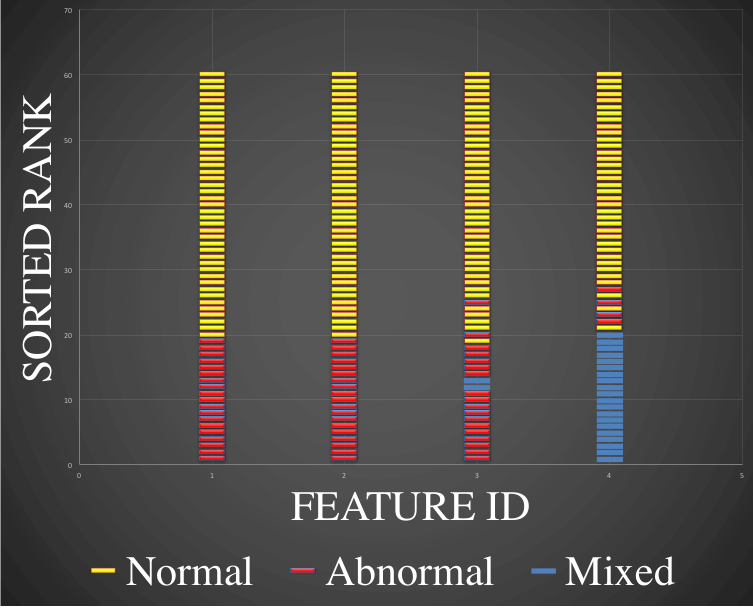
\includegraphics[width=0.5\textwidth]{images/exstreamplot.png}
  \caption{Visualization of the segments of 4 features. The red points are the anomalous points,the yellow points are the normal points and the blue are mixed. Segments are continuous points of the same colour.}
  \label{fig:exstreamplot}
\end{figure}
Originally, Exstream was created to provide a rigorous and formal method for providing short and human readable explanations for anomalies. This method presents the challenge of finding the optimal explanation to an anomaly as a submodular optimization problem. The intuition behind this model is that adding features to our explanation has a diminishing return. This is because the more features we add, the less information new features will provide.\\
Submodular optimisation being NP-hard, a heuristice was therefore introduced to solve the problem. This method relies on Entropy to compute single feature scores.\\\\
We start with two sets of points $S_a$ and $S_n$ containing respectively the anomalous and normal points.
For each feature $f_i$, we will sort the points in $S_a$ and $S_n$ and merge them into one set. We will then define segments on this set as neighbouring points of the same class.

We will compute a segmentation entropy defined as follows:
If there are n segmentations, and $p_i$ represents the ratio of data points included in the ith segmentation, the segmentation entropy is:
\begin{equation}
    H_{segmentation} = \sum_{i=1}^{n} p_i \log(\frac{1}{p_i})
\end{equation}

Exstream was originally aimed at categorical data. Therefore there can be features with values that belong both to anomaly and to normal points. We need to penalize these features. This is done by giving the worst score to those points of mixed class. Let $c_i$ be a mixed interval and $c_i^*$ be the segment rearanged in its worst ordering.\\
Then the maximum entropy is defined as:
\begin{equation}
    H_{max} = \sum_{i=1}^{n} H_{segmentation}(c_i^*)
\end{equation}
Finally, we normalize the score by the class entropy to get a values between 0 and 1. The class entropy is defined as follows:
Let $|S_a|$ and $|S_n|$ be the number of points in $S_a$ and $S_n$ respectively. $p_a = \frac{|S_a|}{|S_a| + |S_n|}$ and $p_n = \frac{|S_n|}{|S_a| + |S_n|}$. The class entropy is then:
\begin{equation}
    H_{class} = p_a \log(\frac{1}{p_a}) + p_n \log(\frac{1}{p_n})
\end{equation}

The final score for a feature is then:
\begin{equation}
    score(f_i) = \frac{H_{segmentation} + H_{max}}{H_{class}}
\end{equation}
This score reflects the segmentation of the feature with respect to anomaly and normal classes. The higher the score, the more separated normal and anomaly classes are. For example a feature with a score of 1 would have all the anomaly points in one segment and all the normal points in another. As we can see on \autoref{fig:exstreamplot}, the first two features have a score of 1. The third a score of 0.31 and the fourth 0.18.\\


Exstream selects the best features based on reward leap filtering. It also provides methods to filter out redundant features using correlation clusters. It also removes "false positive" features which are defined as those with excessively large standard deviation or that tend to only increase or decrease on both the normal and anomalous interval.\\

\subsubsection{Exstream using Bins}
An attempt to improve Exstream was made by Mija Pilkaite during her Bachelor thesis \cite{MijaExstream}. The first idea was to use bins to discretize the data. This would make the method more suited for continuous data. Each feature values would be divided into b bins. Each bin would be marked as either Normal, Anomalous or Mixed. The entropy would then be computed on these bins instead of points. 
The second idea was to reduce uncertainty in the anomalous interval boundaries. Even when using ground truth segments with anomalous intervals marked by hand, there in always some uncertainty as to exact endpoints of the intervals. \\
In order to minimize this labeling uncertainty, the points would have different weights in the computation of the entropy depending on their position in the trace. This weighting would be done using a Gaussian distribution centered around the middle of the interval as such:
% Equation
\[
w_t =
\begin{cases}
\exp \left( - \left( \frac{| position - \frac{interval\_length}{2} |}{\sigma \times \frac{interval\_length}{100}} \right)^{\beta} \right), & \text{if } 0 \leq position \leq interval\_length \\
0, & \text{otherwise}
\end{cases}
\]
This was further worked on by Clement Martineau who fixed some issues and made the method work better in higher dimensions.\\
\subsubsection{Metrics}
The Exathlon pipeline provides a set of metrics to evaluate the performance of the explanation models. These metrics are the following:
\begin{enumerate}
  \item ED1: These metrics are based on local behavior of the anomaly explanation.
  \begin{itemize}
    \item Time: The time taken to compute the explanation.
    \item Size: The size of the explanation. This is the number of features contained in the explanation.
    \item Perturbed Size: Size of the explanation after perturbation. A perturbation is defined as a random sampling of 80\% of the data in the normal and anomalous intervals. The perturbed size is the number of features in the explanation of a trace having been perturbed.
    \item Instability: A measure of the difference in the explanation before and after a perturbation. A high instability means that the explanation isn't locally stable.
    \item F1 Score, Precision, Recall: These metrics are computed by getting an explanation on a randomly sampled 80\% of the normal and anomalous dat and then testing the explanation on the remaining 20\%. The testing is done on the intervals being returns as being anomalous. From them a Precision and Recall score are computed. The F1 Score is the harmonic mean of the two. Similarly as for the instability, the random sampling and evaluation are carried out 5 times and the average is taken.
  \end{itemize}
  \item ED2: These metrics are based on global behavior of the anomaly explanation.
  \begin{itemize}
    \item Discordance: This is the degree of disagreement between the explanation for anomalies of the same type. This measure is computed for each type of anomaly as the entropy of the number of each feature found in all explanations of this type. Then taking two to that power and normalizing by the average number of features in the explanations.
    \item F1 Score, Precision, Recall: these metrics are computed by getting an explanation on one sample and evaluating it on all the other test samples. Similarly as for ED1, these scored are computed on the intervals being returned as being anomalous. The F1 Score is the average of the F1 Scores computed on each other test sample.
  \end{itemize}

\end{enumerate}
These metrics are all computed for each type of anomaly as well as for the whole dataset.\\
It is important to note the limitations of these metrics. For anomaly explanation contrary to anomaly detection, there is no ground truth. Therefore getting perfect Discordance and Stability does not imply that the explanation is good. For example a method returning \textit{feature1} as an explanation everytime would get perfect scores for both metrics. This is especially important for explanation methods that do not provide intervals but only important features. This is why inspecting specific examples and determining if the explanation provided is relevant is important.\\
Another limitation comes from ED2 F1 score, Precision and Recall. As stated in \autoref{subsec:divad_domain}, the domain of the trace being considered is important. A point that could be considered an anomaly in one domain could be normal in another. Therefore an interval being selected as an explanation in one domain could be considered normal in another. The fact that we compare explanations against all other test samples means that we are comparing explanations from different domains. This property of our data significantly undermines the importance of these metrics.
We can even go further and state that the existence of different domains in our data undermines the global consistency of our anomaly explanator, at least when it comes to intervals.\\\\
These metrics are usefull in comparing anomaly explanation methods. However, quantifying the importance of each is difficult. Especially when considering metrics such as Discordance and Instability. The way these metrics is computed is arbitrary and their interpretation is not straightforward. This is especially true for Discordance when being normalize, we raise two to the power of the entropy score and divide by the average number of features in an explanation. These manipulations cloud the interpretation of the metric and the way it would change when adding or removing features.\\\\
Overall, these metrics are very usefull in comparing different methods. However, they should be taken with a grain of salt and the results should be interpreted with caution\\  

\section{Improving the sample set}

\section{Generalizing Exstream to Higher dimensions}
\subsection{Submodular optimization}
\subsection{Methods for generalizing Entropy}
\subsubsection{Boxes}
\subsubsection{KNN}
\subsubsection{Decision Trees}
\section{Conclusion}

\newpage
\bibliographystyle{plain}
\bibliography{main}

\newpage
\appendix

\section{Appendix}
\label{sec:appendix}


\begin{figure}[h]
    \centering
    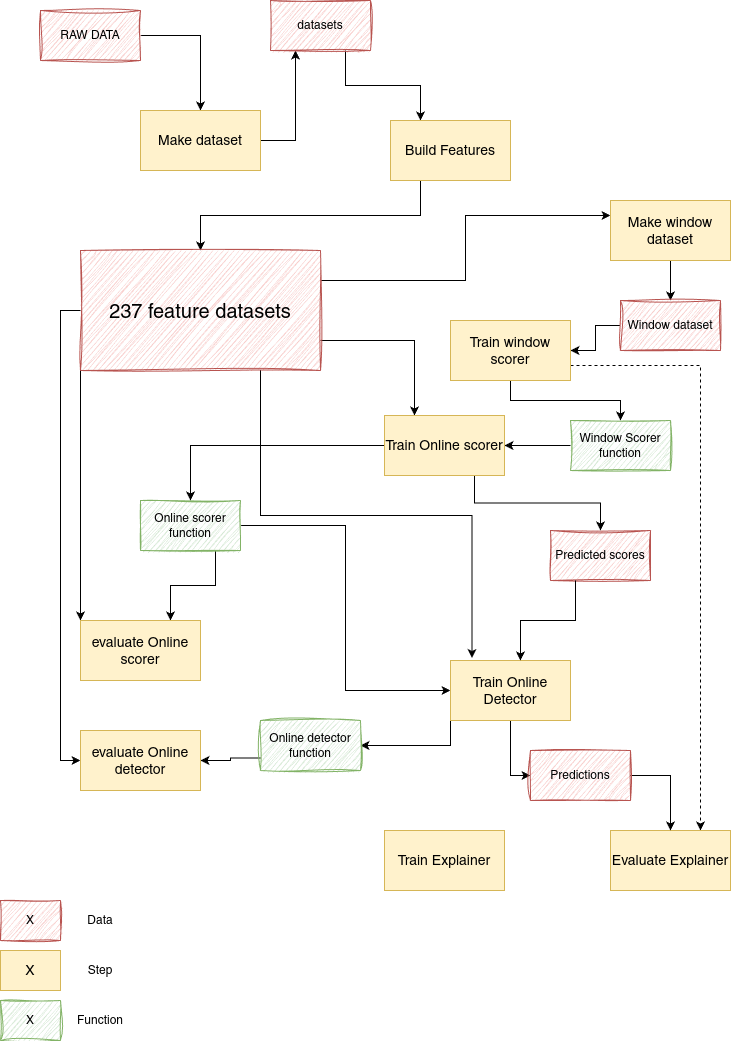
\includegraphics[width=0.7\textwidth]{images/pipeline.drawio.png} % Replace with your image file name
    \caption{Pipeline of Exathlon}
    \label{fig:pipeline}
\end{figure}
\end{document}
